% Supplementary Material — HeartLens TinyML ECG (single-column, not counted in 6-page limit)
\documentclass[10pt, conference, letterpaper]{IEEEtran}
\usepackage{amsmath,amssymb,booktabs,graphicx,hyperref}
\usepackage[table]{xcolor}
\setlength{\dbltextfloatsep}{8pt plus 2pt minus 2pt}
\begin{document}
\title{Supplementary Material:\\Patient-Independent TinyML ECG Classification --- Per-Fold Support, Noise, and Calibration Details}
\author{HeartLens --- Supplement to Main Paper (6 pages)}
\maketitle
This supplement provides the per-fold numbers referenced in the main paper (\texttt{results/folds\_5x2.json}, frozen 5$\times$2, Seeds 0,1). It is \emph{not} counted in the 6-page limit. Main Figs.~4--5 and Tables~II--VI stay in the main paper; Figs.~S1--S4 below were deferred to meet the limit.

\section{Frozen Patient-Disjoint Folds}
48 MIT-BIH records, \texttt{Patients$_{\rm train}\cap$Patients$_{\rm test}=\emptyset$}. Each of 10 test folds is listed with its record IDs and test support (N/APB/V windows, 1-s centered on R-peaks, 360 samples).
\begin{table}[h]
\centering
\caption{Frozen folds (\texttt{heart-lens-training/results/folds\_5x2.json})}
\label{tab:supp-folds}
\footnotesize
\begin{tabular}{ccl c}
\toprule
Seed & Fold & Test records & N / APB / V (windows)\\
\midrule
0&0&101,102,104,112,119 & 587 / 2 / 232\\
0&1&103,106,111,117,124 & 466 / 138 / 304\\
0&2&100,108,118,200,201 & 672 / 502 / 602\\
0&3&107,109,113,114,203 & 473 / 32 / 362\\
0&4&105,115,116,208,210 & 802 / 38 / 769\\
1&0&103,106,116,200,202 & 775 / 152 / 502\\
1&1&100,107,109,117,122 & 631 / 25 / 458\\
1&2&101,112,118,121,123 & 659 / 482 / 426\\
1&3&102,104,113,115,203 & 380 / 1 / 566\\
1&4&105,108,111,114,119 & 555 / 52 / 317\\
\bottomrule
\end{tabular}
\end{table}
APB support 1--502/fold explains the high variance in Table~II in the main paper; two folds $\le$2 APB windows make per-fold APB F1 undefined/0 (mean-of-folds unstable). Pooled-confusion macro 0.643 (both CNN/TCN) is reported alongside mean-of-folds 0.619/0.615 in the main text.

\section{Per-Fold F1 and Support (Grouped CV)}
All four architectures share identical folds (paired). Raw per-fold JSON: \texttt{heart-lens-training/results/group\_kfold\_ckpt/\{cnn,tcn,lstm,gru\}\_s\{seed\}\_f\{fold\}.json}. Below: support (windows) and F1 (Normal/APB/PVC) + macro.

\begin{table}[h]
\centering
\caption{CNN --- per-fold F1 and support (macro mean 0.619$\pm$0.242)}
\label{tab:supp-cnn}
\footnotesize
\begin{tabular}{cc c c c}
\toprule
Seed & Fold & Support N/APB/V & F1 N / APB / PVC & Macro\\
\midrule
0&0&587/2/232&0.977/0.000/0.956&0.644\\
0&1&466/138/304&0.877/0.837/0.907&0.874\\
0&2&672/502/602&0.549/0.000/0.000&0.183\\
0&3&473/32/362&0.866/0.596/0.865&0.776\\
0&4&802/38/769&0.958/0.000/0.972&0.643\\
1&0&775/152/502&0.969/0.866/0.986&0.940\\
1&1&631/25/458&0.930/0.000/0.936&0.622\\
1&2&659/482/426&0.592/0.000/0.000&0.197\\
1&3&380/1/566&0.799/0.000/0.841&0.547\\
1&4&555/52/317&0.890/0.535/0.866&0.764\\
\bottomrule
\end{tabular}
\end{table}

\begin{table}[h]
\centering
\caption{TCN --- per-fold F1 and support (macro mean 0.615$\pm$0.229)}
\label{tab:supp-tcn}
\footnotesize
\begin{tabular}{cc c c c}
\toprule
Seed & Fold & Support N/APB/V & F1 N / APB / PVC & Macro\\
\midrule
0&0&587/2/232&0.988/0.000/0.974&0.654\\
0&1&466/138/304&0.788/0.732/0.851&0.790\\
0&2&672/502/602&0.551/0.000/0.026&0.192\\
0&3&473/32/362&0.886/0.474/0.914&0.758\\
0&4&802/38/769&0.961/0.000/0.970&0.644\\
1&0&775/152/502&0.970/0.864/0.983&0.939\\
1&1&631/25/458&0.922/0.000/0.916&0.612\\
1&2&659/482/426&0.592/0.000/0.000&0.197\\
1&3&380/1/566&0.877/0.100/0.935&0.637\\
1&4&555/52/317&0.902/0.400/0.890&0.730\\
\bottomrule
\end{tabular}
\end{table}

\begin{table}[h]
\centering
\caption{LSTM --- per-fold F1 and support (macro mean 0.582$\pm$0.096)}
\label{tab:supp-lstm}
\footnotesize
\begin{tabular}{cc c c c}
\toprule
Seed & Fold & Support N/APB/V & F1 N / APB / PVC & Macro\\
\midrule
0&0&587/2/232&0.955/0.000/0.895&0.617\\
0&1&466/138/304&0.694/0.567/0.675&0.645\\
0&2&672/502/602&0.659/0.008/0.809&0.492\\
0&3&473/32/362&0.688/0.161/0.696&0.515\\
0&4&802/38/769&0.944/0.048/0.960&0.650\\
1&0&775/152/502&0.886/0.599/0.899&0.795\\
1&1&631/25/458&0.784/0.035/0.697&0.505\\
1&2&659/482/426&0.659/0.000/0.689&0.449\\
1&3&380/1/566&0.798/0.000/0.854&0.551\\
1&4&555/52/317&0.848/0.164/0.784&0.598\\
\bottomrule
\end{tabular}
\end{table}

\begin{table}[h]
\centering
\caption{GRU --- per-fold F1 and support (macro mean 0.526$\pm$0.170)}
\label{tab:supp-gru}
\footnotesize
\begin{tabular}{cc c c c}
\toprule
Seed & Fold & Support N/APB/V & F1 N / APB / PVC & Macro\\
\midrule
0&0&587/2/232&0.973/0.000/0.921&0.631\\
0&1&466/138/304&0.468/0.397/0.264&0.376\\
0&2&672/502/602&0.657/0.008/0.866&0.511\\
0&3&473/32/362&0.447/0.088/0.173&0.236\\
0&4&802/38/769&0.934/0.000/0.952&0.629\\
1&0&775/152/502&0.914/0.598/0.926&0.813\\
1&1&631/25/458&0.840/0.000/0.803&0.548\\
1&2&659/482/426&0.393/0.016/0.466&0.292\\
1&3&380/1/566&0.769/0.000/0.858&0.542\\
1&4&555/52/317&0.888/0.289/0.864&0.680\\
\bottomrule
\end{tabular}
\end{table}

\section{Deferred Figures (single-column)}
Figs.~S1--S4 were in prior drafts as double-column; they are retained here single-column for completeness. Main paper keeps Figs.~4--5 in the main paper and calibration as primary deployment figures.
\begin{figure}[h]
\centering
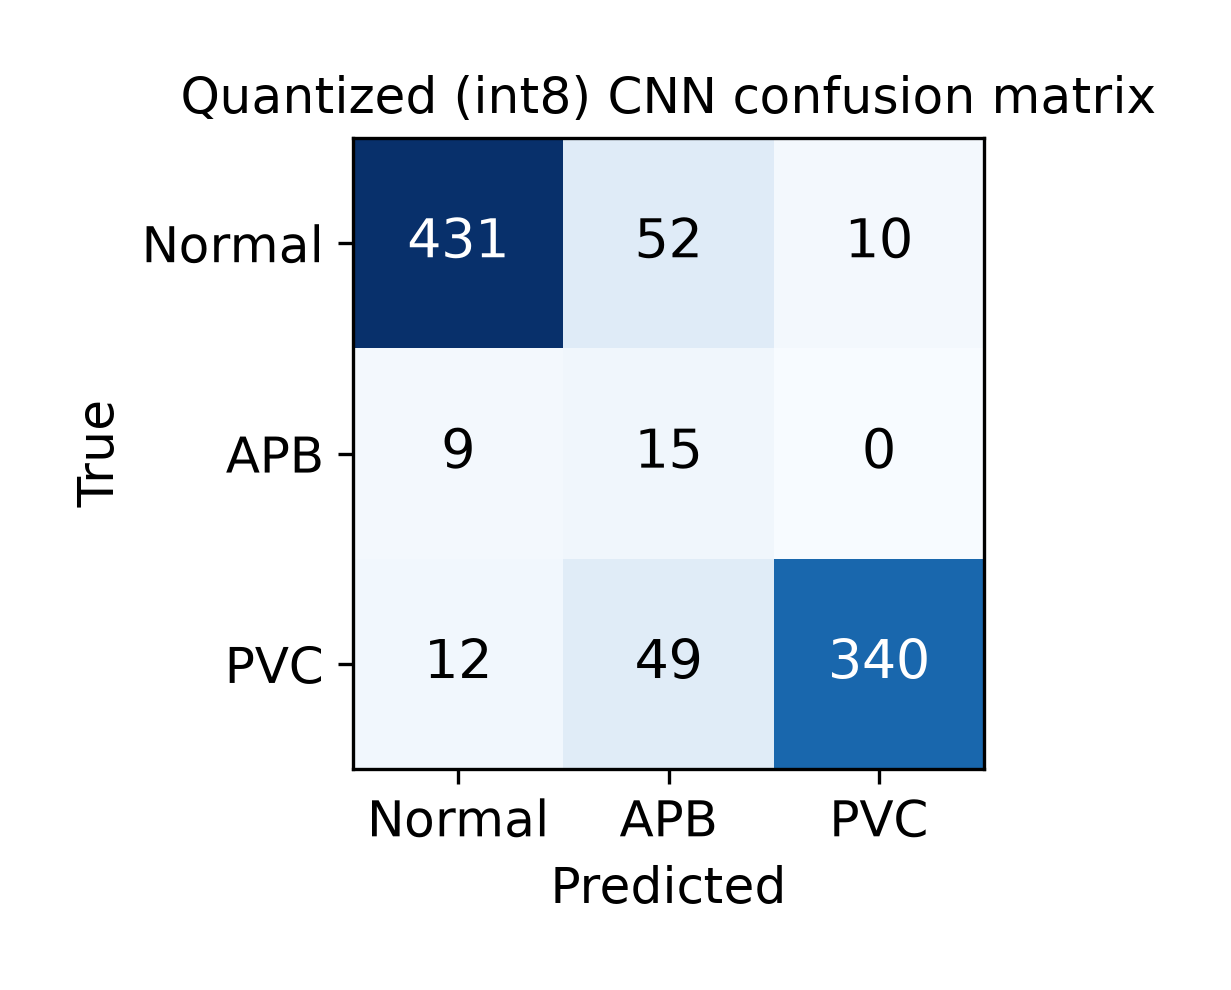
\includegraphics[width=0.90\columnwidth]{figures/fig_confusion.png}
\caption{Confusion matrix (representative fold; supplementary).}
\label{fig:supp-confusion}
\end{figure}
\begin{figure}[h]
\centering
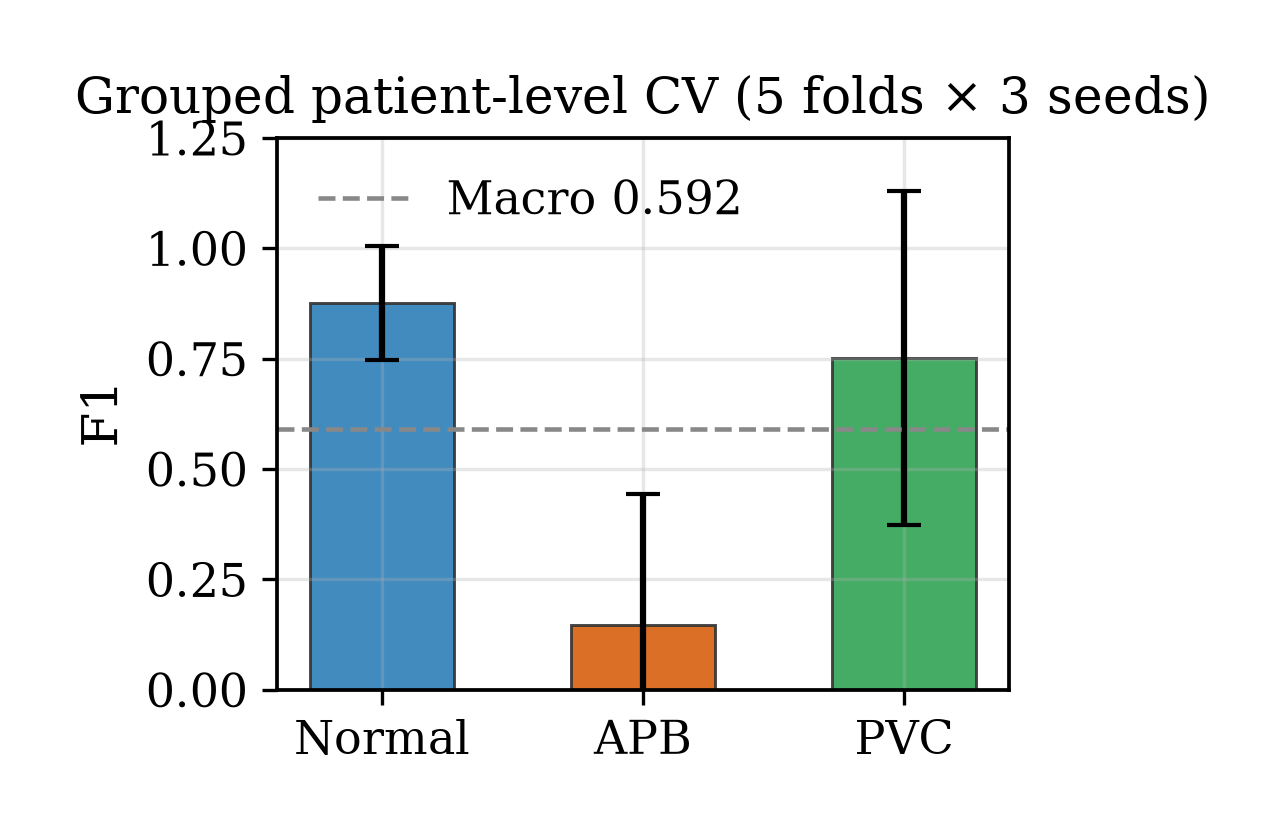
\includegraphics[width=0.90\columnwidth]{figures/fig_gcv.png}
\caption{Grouped-CV macro distribution per architecture (supplementary).}
\label{fig:supp-gcv}
\end{figure}
\begin{figure}[h]
\centering
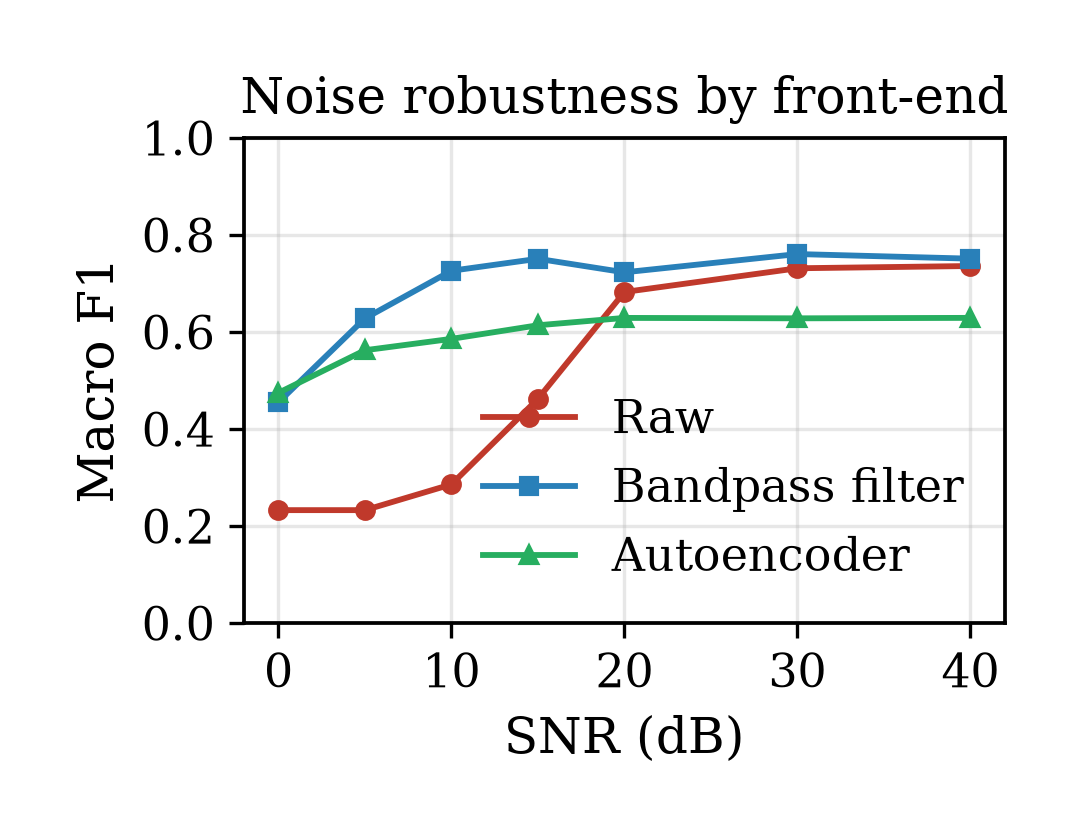
\includegraphics[width=0.90\columnwidth]{figures/fig_noise.png}
\caption{Macro F1 vs SNR averaged over 5 artifacts (supplementary; see Fig.~5 in the main paper for per-artifact split).}
\label{fig:supp-noise}
\end{figure}
\begin{figure}[h]
\centering
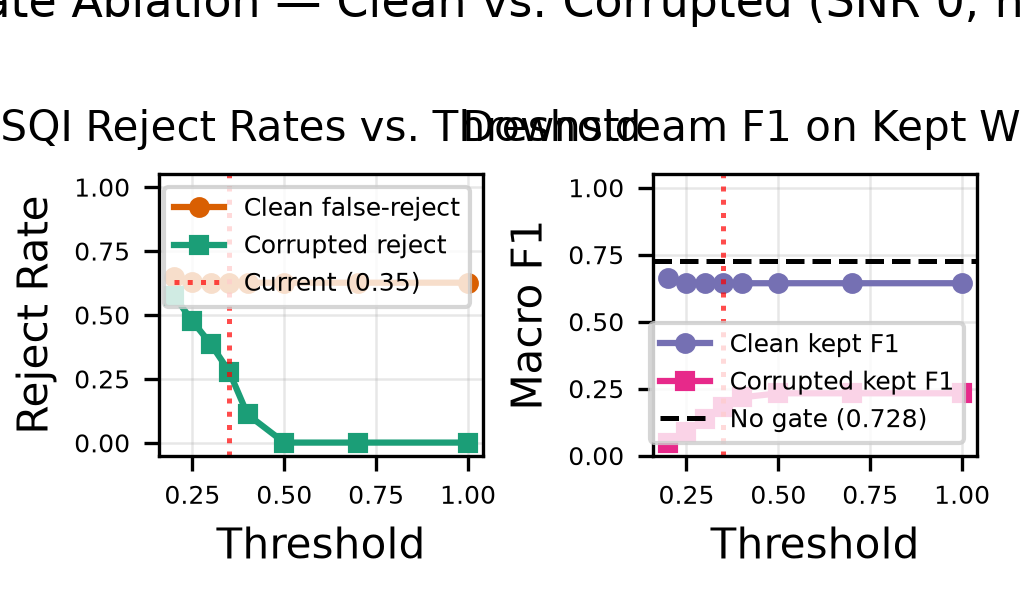
\includegraphics[width=0.90\columnwidth]{figures/fig_sqi.png}
\caption{SQI gate: clean false-reject 62.6\% at 0.35, corrupted reject 27.9\%, downstream macro 0.727$\rightarrow$0.643 --- not deployable (Fig.~S1 in main text).}
\label{fig:supp-sqi}
\end{figure}

\section{Noise Per-Artifact Full Table}
\texttt{heart-lens-training/results/per\_artifact\_noise.json}: macro F1 vs SNR per artifact (Butterworth wins 3/5, raw wins motion, AE only low-SNR PLI).
\begin{table}[h]
\centering
\caption{Per-artifact noise robustness (macro F1; excerpt, see JSON for full 5$\times$7$\times$3).}
\label{tab:supp-per-artifact}
\footnotesize
\begin{tabular}{l l l l l}
\toprule
SNR & Raw & Filter & AE & Artifacts\\
\midrule
0--40\,dB & 0.233--0.736 & 0.455--0.751 & 0.475--0.629 & avg over 5 (Table~III in the main paper in main)\\
\midrule
\multicolumn{5}{l}{\textit{Per-artifact extremes (from per\_artifact\_noise.json):}}\\
BW: raw 0.71--0.75, filter 0.73--0.79, AE 0.62--0.83; motion: raw wins at 10\,dB (0.73 vs 0.68);\\
PLI: AE wins only low-SNR (0.62 at 0\,dB); EMG/mixed: filter dominates.\\
\bottomrule
\end{tabular}
\end{table}

\section{Calibration and Quantization Details}
Main Table~VII in the main paper: same 918-window test split (493/24/401 class balance). FP32 \textit{vs} INT8 (PTQ, 200 train windows, \texttt{TFLITE\_BUILTINS\_INT8}) ECE/NLL/Brier with separate temperatures ($T{=}0.350$, $T_{\rm INT8}{=}5.0$). QAT CNN (5$\times$2, TF-MOT, 3 epochs, \texttt{results/qat\_cnn\_summary.json}): FP32 0.642, PTQ 0.549, QAT 0.584 ($\Delta_{\rm QAT-PTQ}{+}0.036\pm0.085$ $p{=}0.42$, 38\% of PTQ loss, still $-$0.058 vs FP32). QAT for Conv1D required TF-MOT default 8-bit path; standard PTQ is the deployed pipeline.

\section{Reproducibility}
Frozen folds \texttt{results/folds\_5x2.json}, 40+16+40 ckpts in \texttt{results/group\_kfold\_ckpt/} and \texttt{results/qat\_ckpt/} (\texttt{.tmp$\rightarrow$.json} atomic), \texttt{results/calibration\_int8.json}, seeds 0,1, TF 2.21/Keras 3/sklearn. All main tables/figs regenerate via \texttt{run\_experiments.sh} and \texttt{scripts/round3\_*.py}.

\end{document}
